%%%%%%%%%%%%%%%%%%%%%%%%%%%%%%%%%%%%%%%%%%%%%%%%%%%%%%%%%%%%%%%%%%%%%%%%%%%%%%%%%%%%%%%%%%%%%
%%%%%%%%%%%%%%%%%%%%%%%%%%%%%%%        Diagramas              %%%%%%%%%%%%%%%%%%%%%%%%%%%%%%%
%%%%%%%%%%%%%%%%%%%%%%%%%%%%%%%%%%%%%%%%%%%%%%%%%%%%%%%%%%%%%%%%%%%%%%%%%%%%%%%%%%%%%%%%%%%%%

\chapter{Diagramas}

\begin{figure}[h]
	\begin{center}
		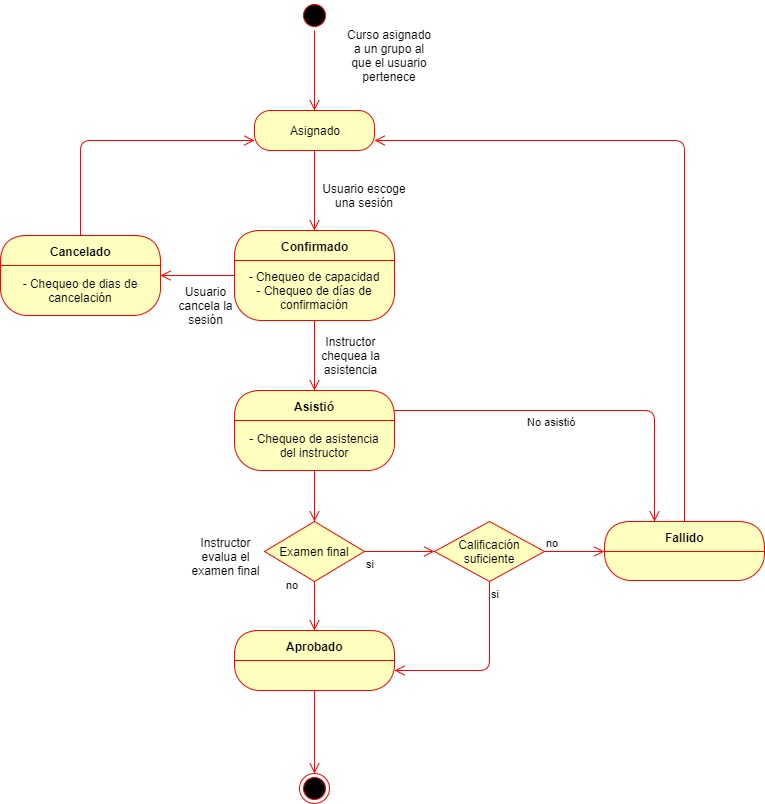
\includegraphics[width=0.9\textwidth]{figuras/diagramaEstadosSesion.jpg}
		\caption{Diagrama que demuestra los distintos estados en los que se puede encontrar una sesión prensencial.} \label{fig:diagramaEstadosSesion}
	\end{center}
\end{figure}

\begin{figure}[h]
	\begin{center}
		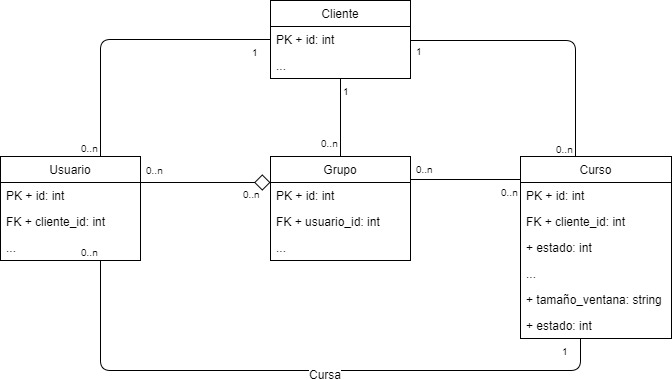
\includegraphics[width=0.9\textwidth]{figuras/databasePrevia.jpg}
		\caption{Diagrama UML parcial de la base de datos del SGA de FKC previa al proyecto.} \label{fig:baseDeDatosPrevia}
	\end{center}
\end{figure}

\begin{figure}[h]
	\begin{center}
		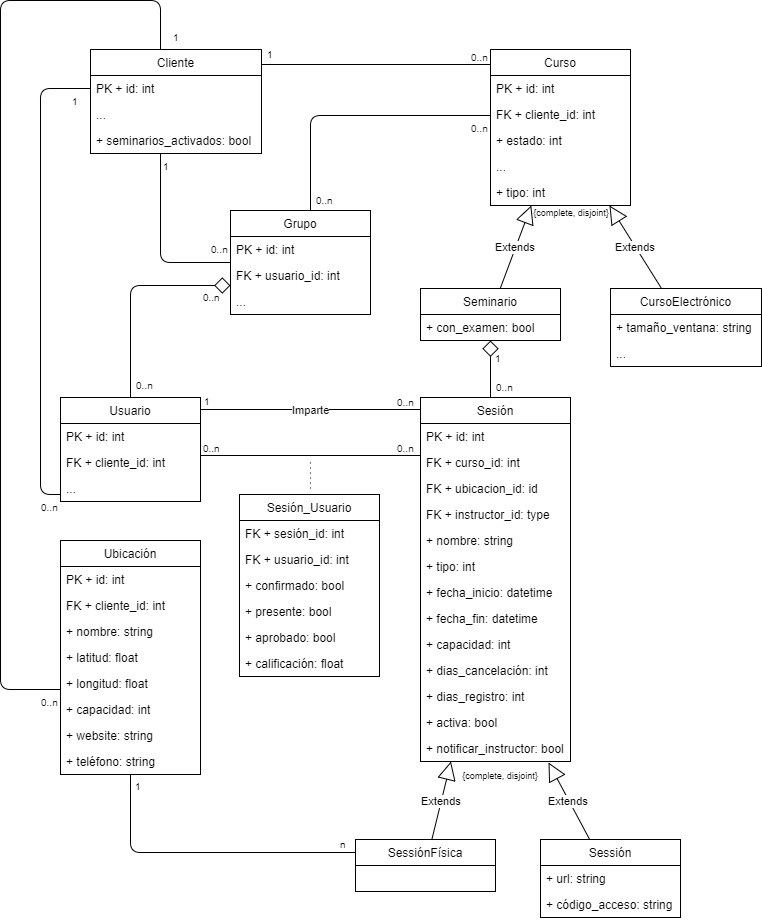
\includegraphics[width=\textwidth]{figuras/database.jpg}
		\caption{Diagrama UML parcial de la base de datos final del SGA de FKC.} \label{fig:baseDeDatosFinal}
	\end{center}
\end{figure}

\begin{figure}[h]
	\begin{center}
		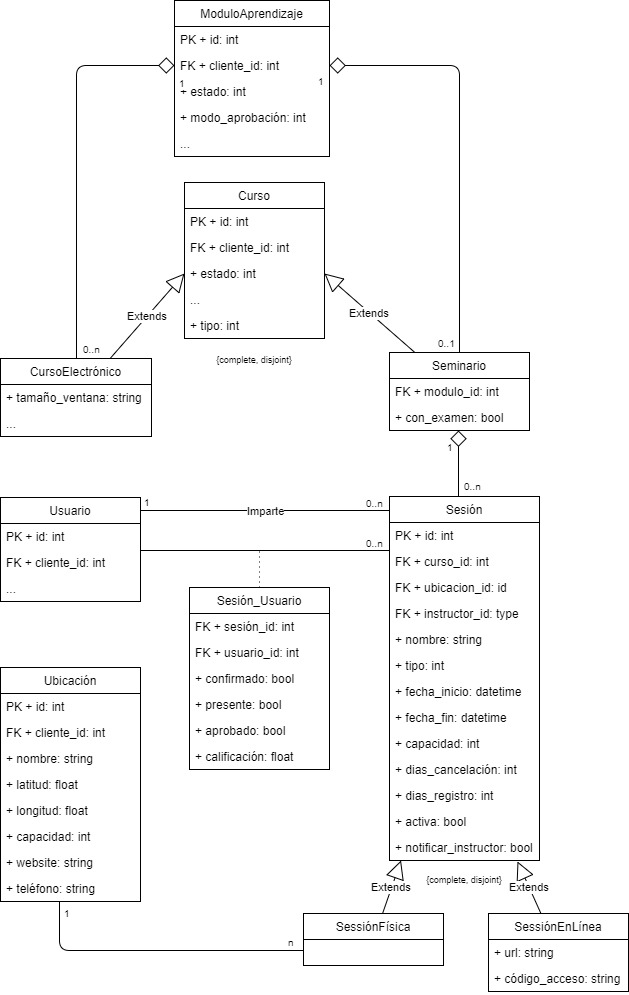
\includegraphics[width=0.8\textwidth]{figuras/databaseBibliomed.jpg}
		\caption{Diagrama UML parcial de la base de datos final del SGA de Bibliomed.} \label{fig:baseDeDatosBibliomed}
	\end{center}
\end{figure}

%%%%%%%%%%%%%%%%%%%%%%%%%%%%%%%%%%%%%%%%%%%%%%%%%%%%%%%%%%%%%%%%%%%%%%%%%%%%%%%%%%%%%%%%%%%%%
%%%%%%%%%%%%%%%%%%%%%%%%%%%%%%%        Screenshots            %%%%%%%%%%%%%%%%%%%%%%%%%%%%%%%
%%%%%%%%%%%%%%%%%%%%%%%%%%%%%%%%%%%%%%%%%%%%%%%%%%%%%%%%%%%%%%%%%%%%%%%%%%%%%%%%%%%%%%%%%%%%%

\chapter{Screenshots de los sistemas}


\begin{figure}[h]
	\begin{center}
		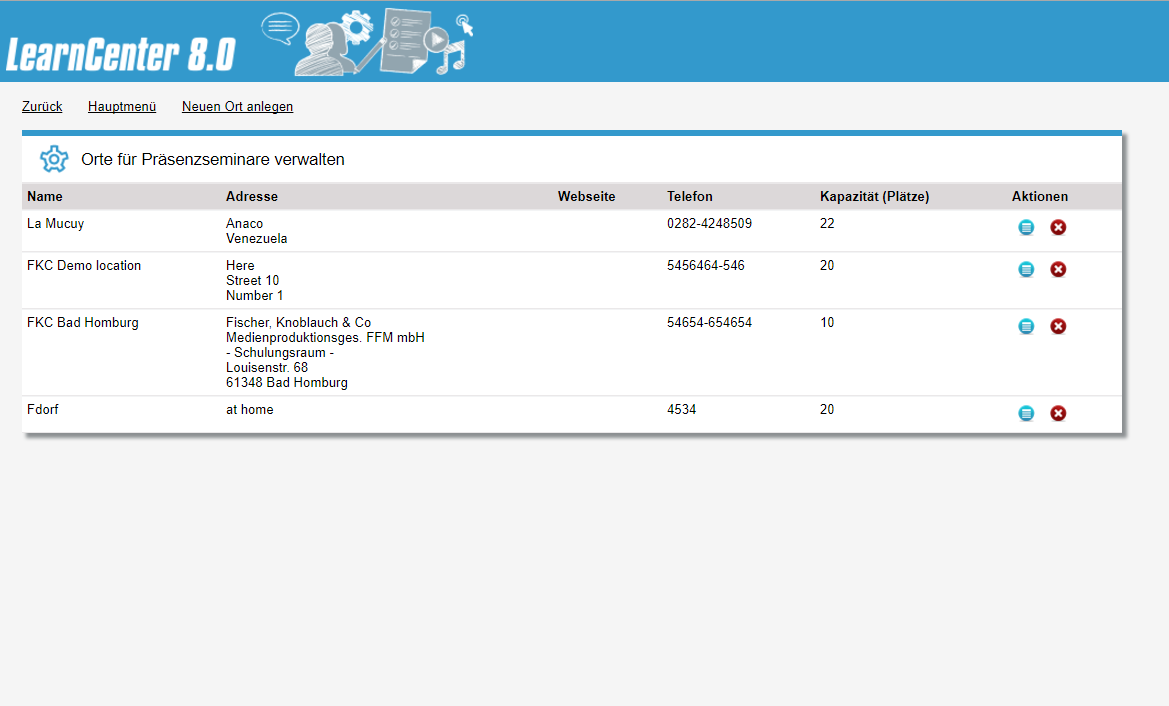
\includegraphics[width=\textwidth]{screenshots/listar_ubicaciones.png}
		\caption{Vista del listado de Ubicaciones.} \label{fig:listarUbicaciones}
	\end{center}
\end{figure}

\begin{figure}[h]
	\begin{center}
		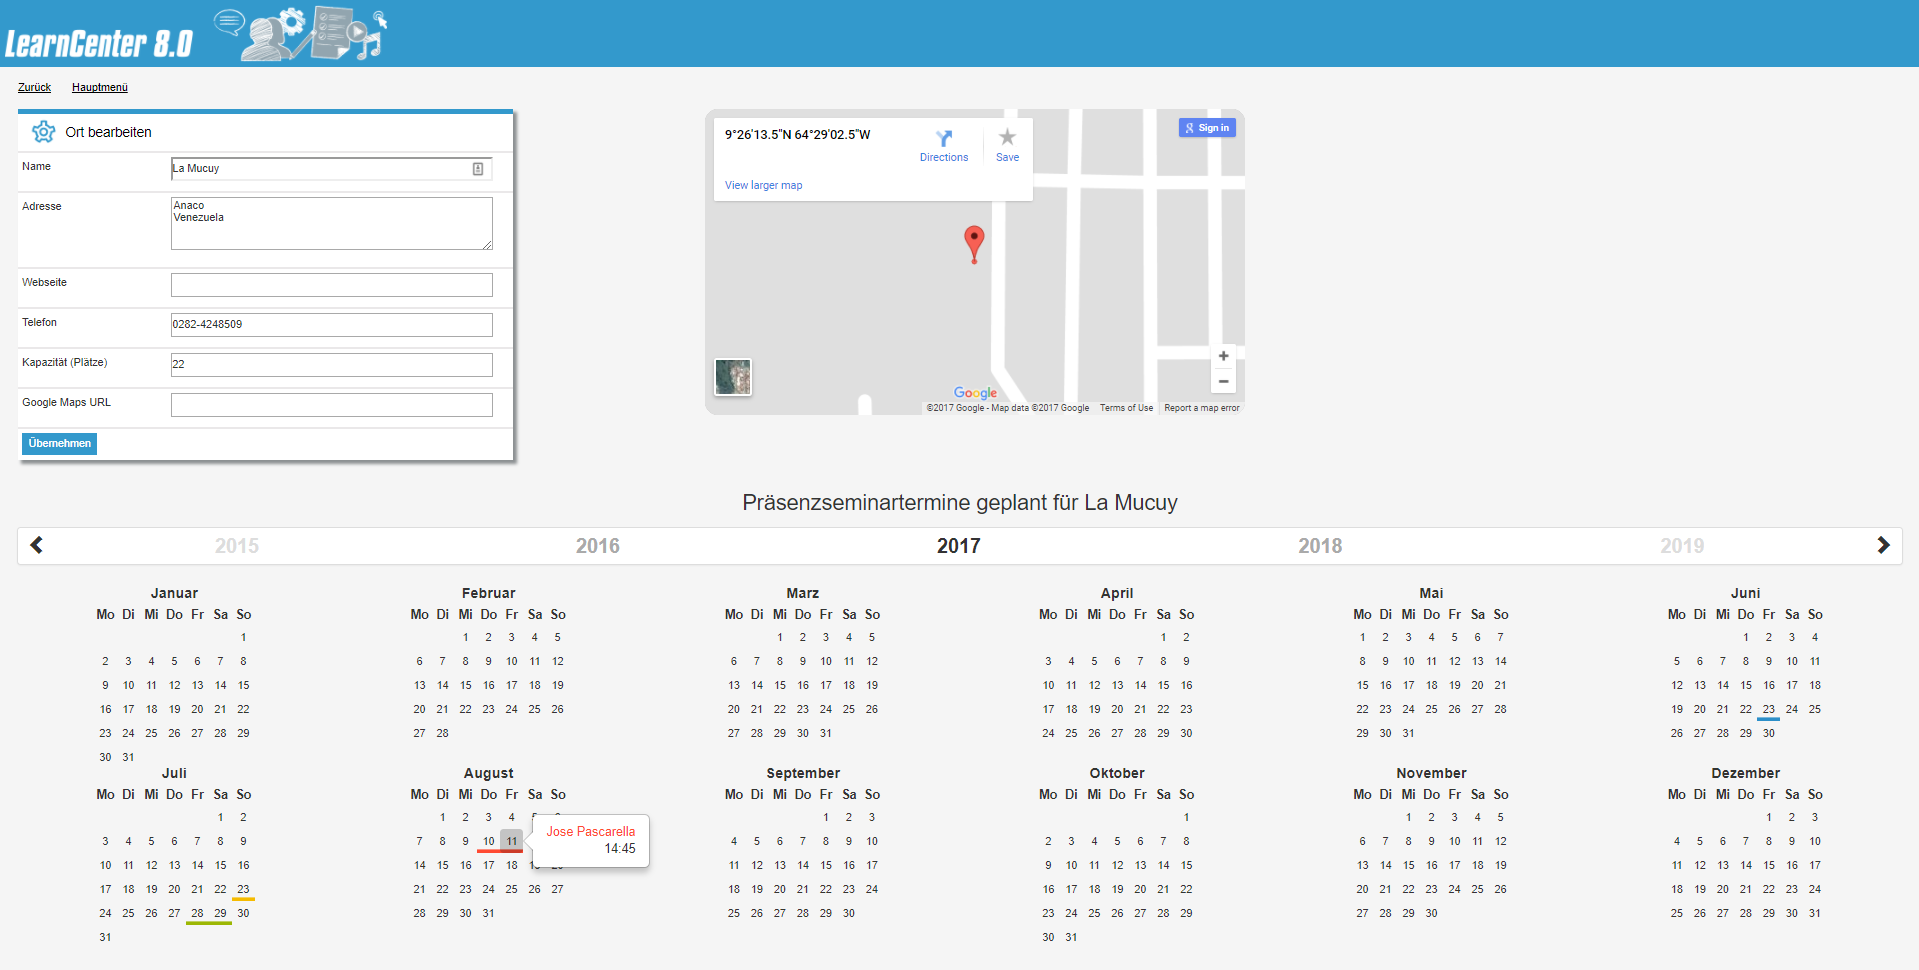
\includegraphics[width=\textwidth]{screenshots/edicion_ubicacion.png}
		\caption{Vista de la edición de una ubicación.} \label{fig:editarUbicaciones}
	\end{center}
\end{figure}

\begin{figure}[h]
	\begin{center}
		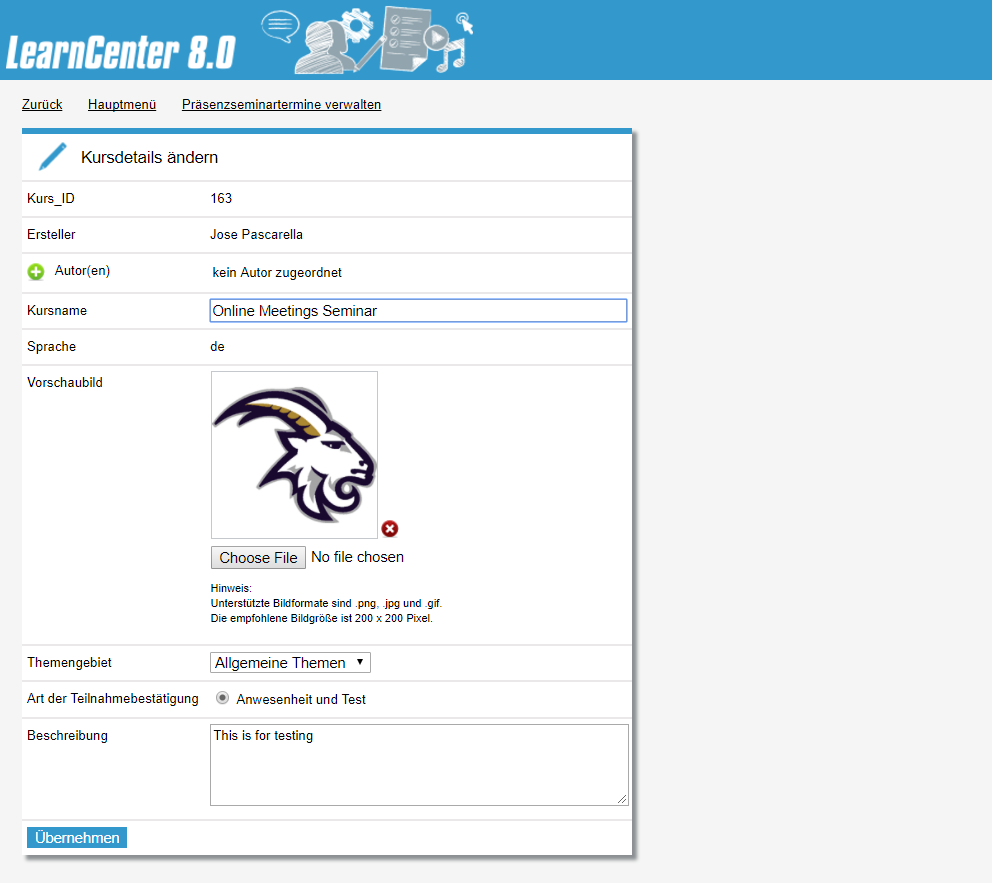
\includegraphics[width=\textwidth]{screenshots/creacion_seminario.png}
		\caption{Vista de la creación de un seminario.} \label{fig:creacionSeminario}
	\end{center}
\end{figure}

\begin{figure}[h]
	\begin{center}
		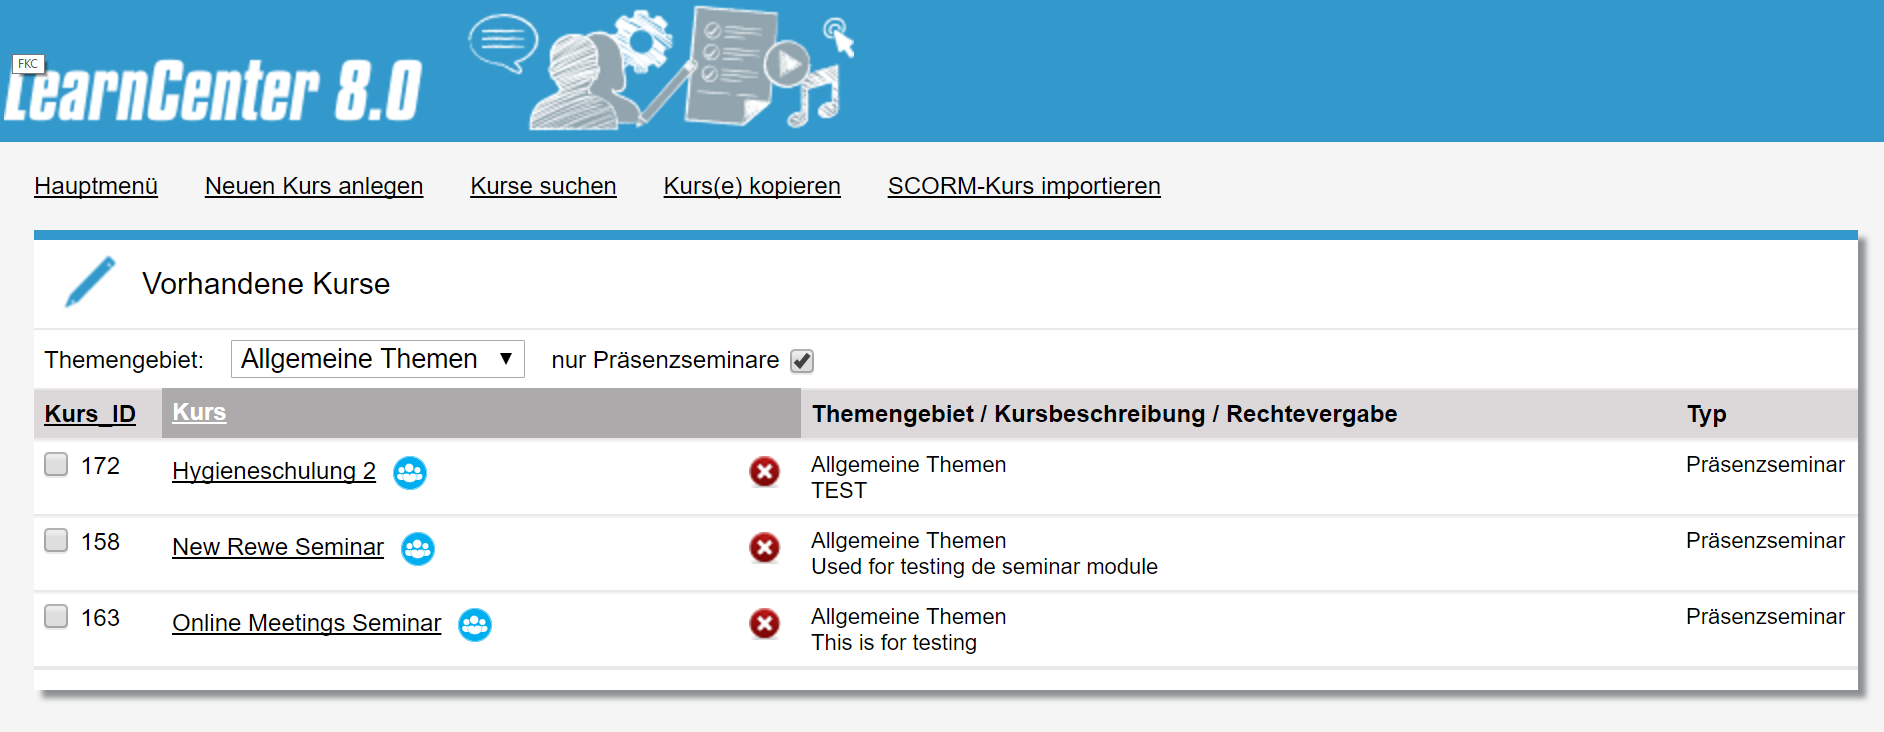
\includegraphics[width=\textwidth]{screenshots/admin_listar_cursos.png}
		\caption{Vista del listado de cursos del sistema para el administrador.} \label{fig:listarCursos}
	\end{center}
\end{figure}

\begin{figure}[h]
	\begin{center}
		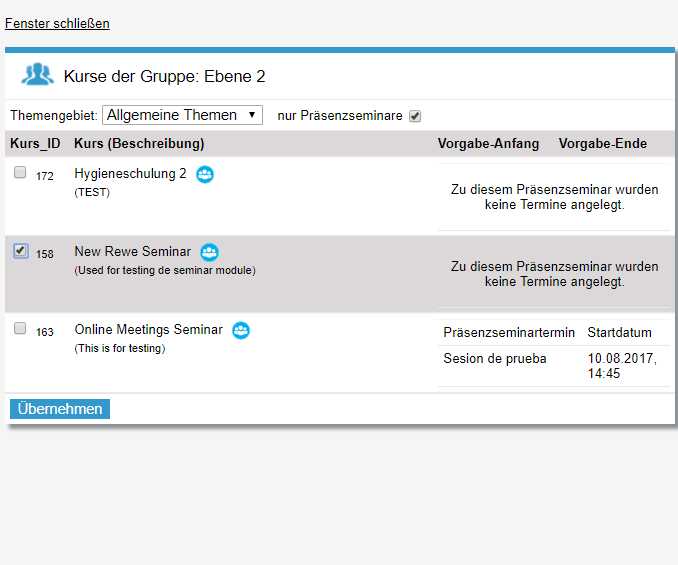
\includegraphics[width=\textwidth]{screenshots/asignar_seminario.png}
		\caption{Vista de la asignación de un seminario a un grupo.} \label{fig:asignarSeminario}
	\end{center}
\end{figure}

\begin{figure}[h]
	\begin{center}
		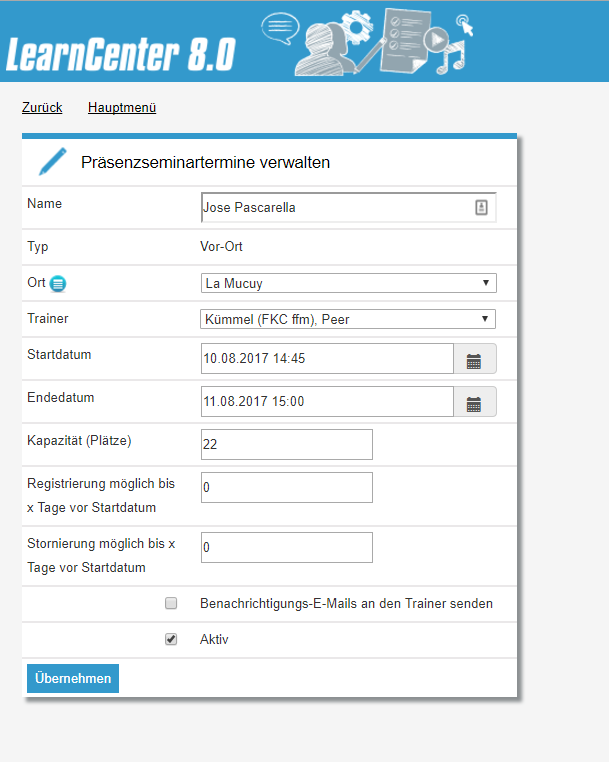
\includegraphics[width=\textwidth]{screenshots/creacion_seminario_sesion.png}
		\caption{Vista de la creación de una sesión de un seminario.} \label{fig:creacionSesion}
	\end{center}
\end{figure}

\begin{figure}[h]
	\begin{center}
		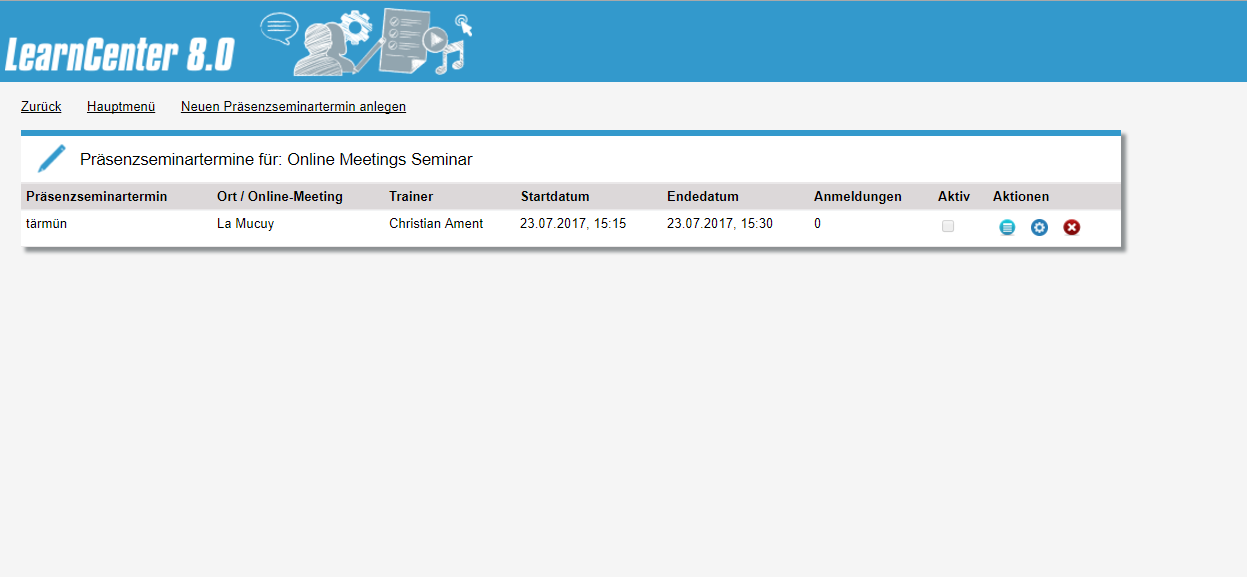
\includegraphics[width=\textwidth]{screenshots/listar_sesiones_seminario.png}
		\caption{Vista del listado de las sesiones de un seminario.} \label{fig:listarSesiones}
	\end{center}
\end{figure}

\begin{figure}[h]
	\begin{center}
		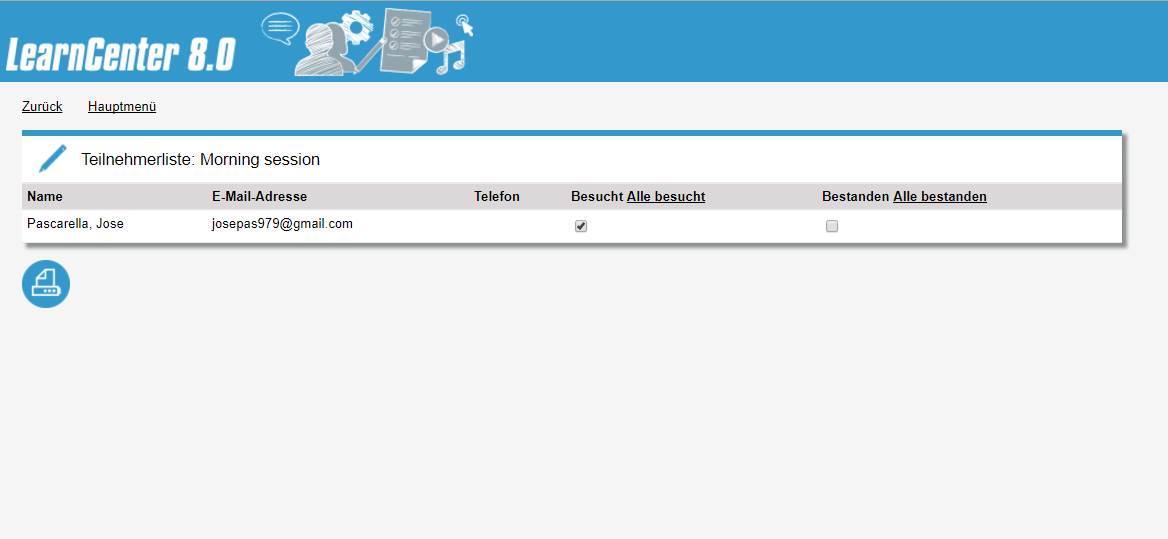
\includegraphics[width=\textwidth]{screenshots/manage_session.png}
		\caption{Vista de los cursos de un instructor.} \label{fig:gestionarSesion}
	\end{center}
\end{figure}

\begin{figure}[h]
	\begin{center}
		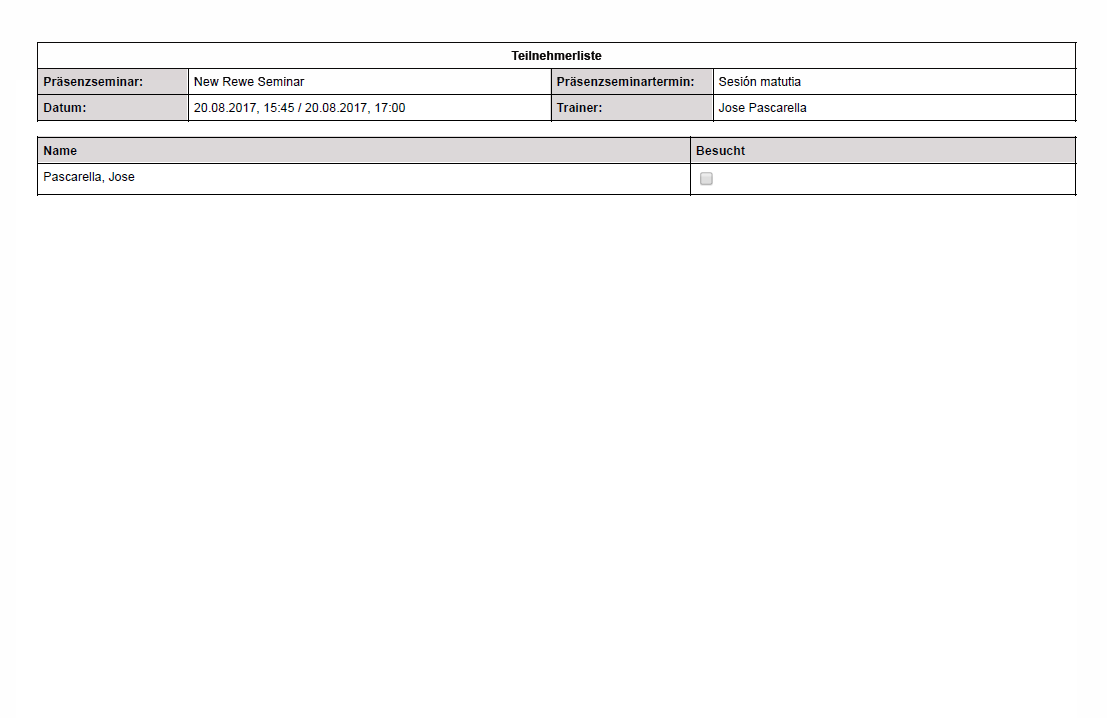
\includegraphics[width=\textwidth]{screenshots/lista_alumnos.png}
		\caption{Archivo PDF generado con la lista de los estudiantes de un curso.} \label{fig:listarAlumnos}
	\end{center}
\end{figure}

\begin{figure}[h]
	\begin{center}
		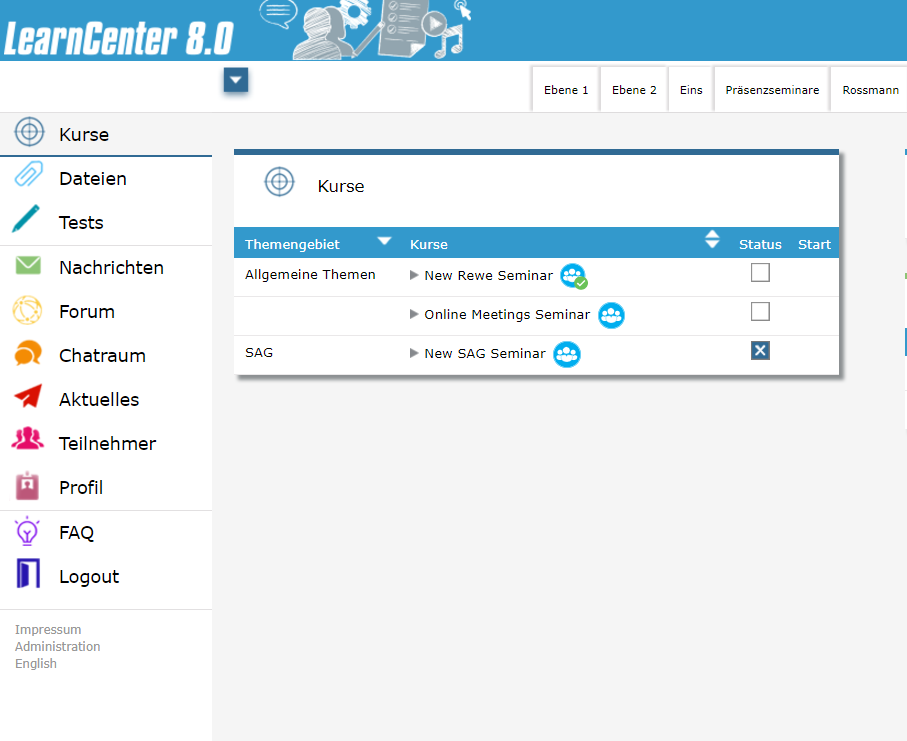
\includegraphics[width=\textwidth]{screenshots/user_listar_cursos2.png}
		\caption{Vista de los cursos disponibles para el usuario aprendiz.} \label{fig:aprendizListarCursos}
	\end{center}
\end{figure}

\begin{figure}[h]
	\begin{center}
		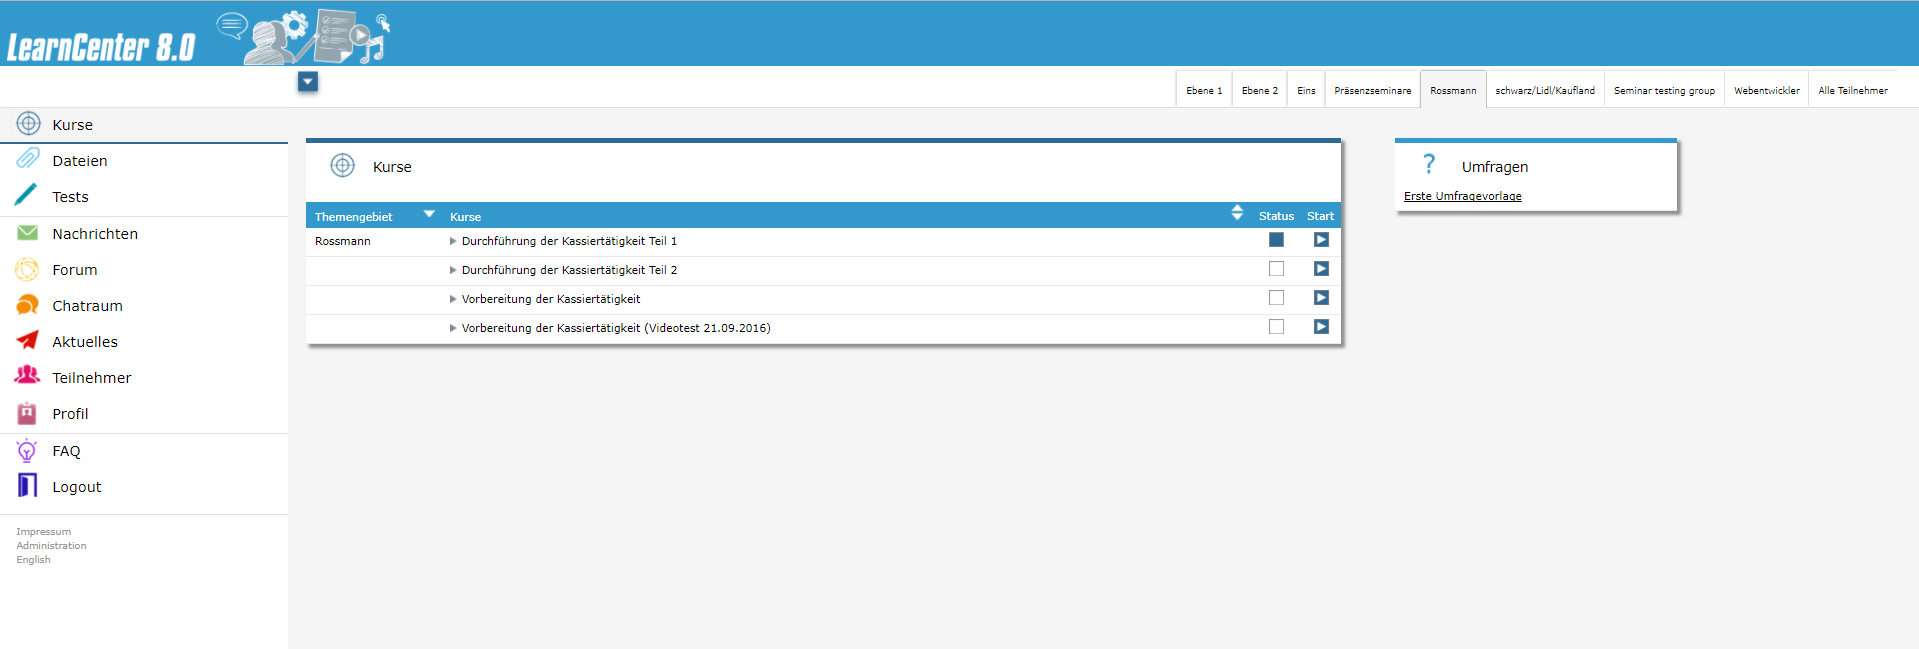
\includegraphics[width=\textwidth]{screenshots/user_listar_seminar_viejo.png}
		\caption{Vista de los cursos disponibles para el usuario aprendiz antes de la extensión realizada en la pasantia.} \label{fig:aprendizListarViejo}
	\end{center}
\end{figure}

\begin{figure}[h]
	\begin{center}
		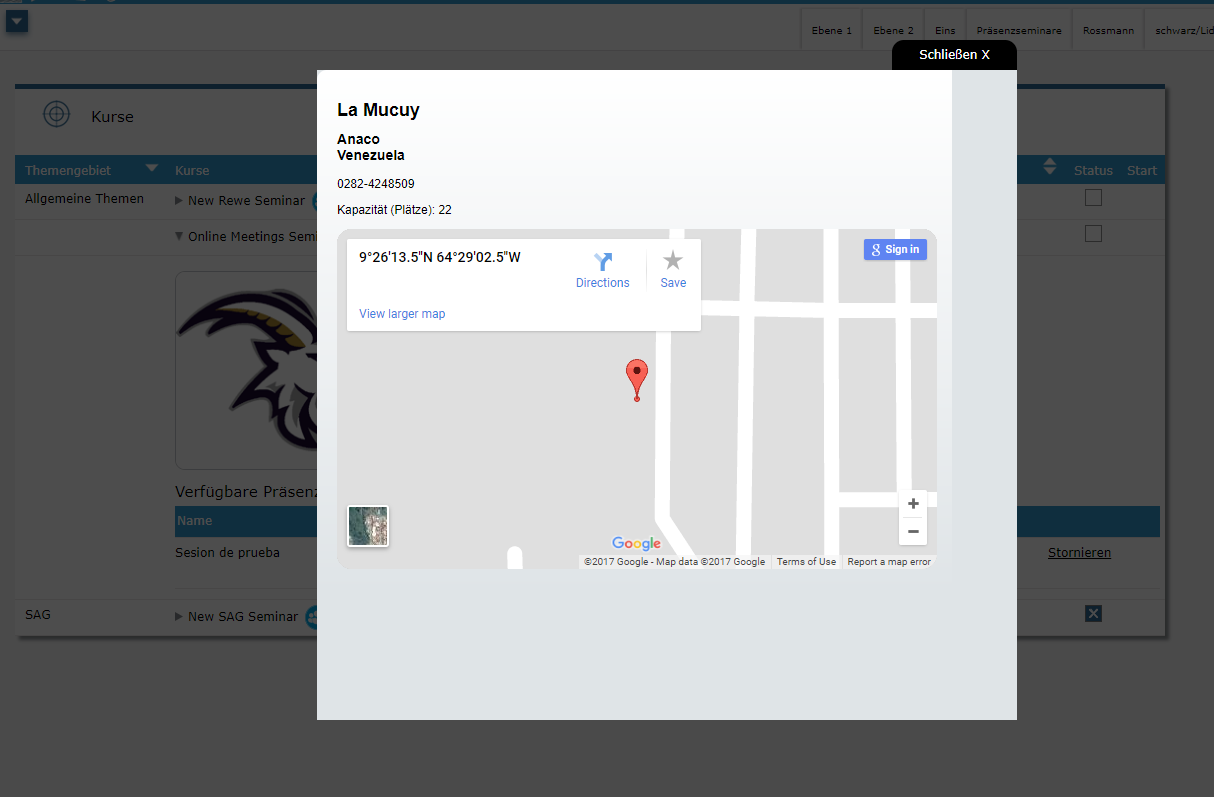
\includegraphics[width=\textwidth]{screenshots/modal_ubicacion.png}
		\caption{Vista del modal mostrado con los datos de la ubicación de la sesión correspondiente.} \label{fig:modalUbicacion}
	\end{center}
\end{figure}

\begin{figure}[h]
	\begin{center}
		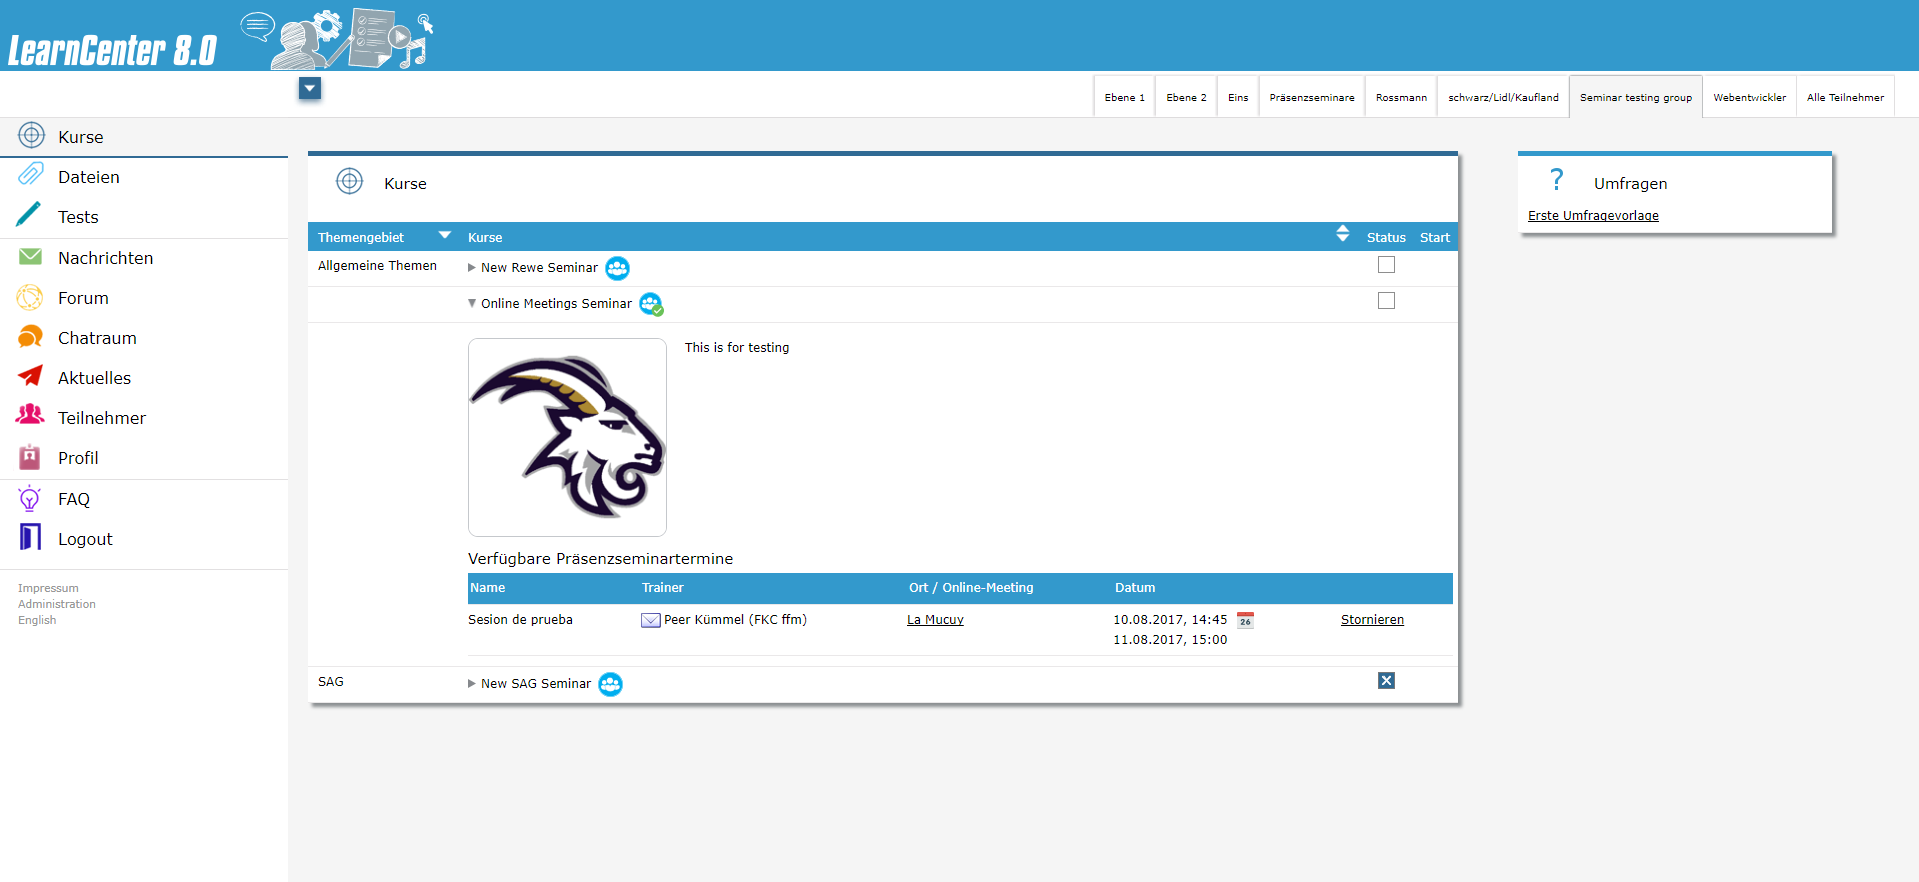
\includegraphics[width=\textwidth]{screenshots/user_reservar.png}
		\caption{Vista de una sesión confirmada por el usario.} \label{fig:usuarioSesionConfirmada}
	\end{center}
\end{figure}

\begin{figure}[h]
	\begin{center}
		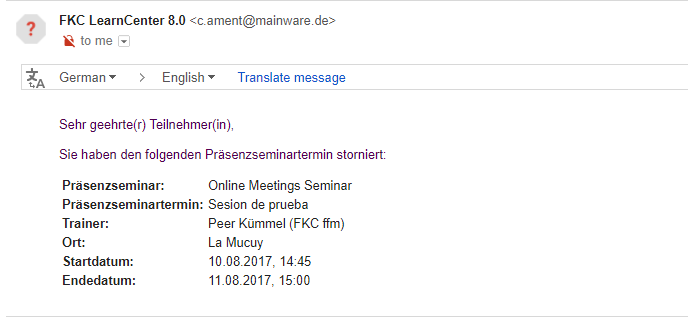
\includegraphics[width=\textwidth]{screenshots/emails.png}
		\caption{Formato de los correos enviados por el sistema.} \label{fig:correos}
	\end{center}
\end{figure}

\begin{figure}[h]
	\begin{center}
		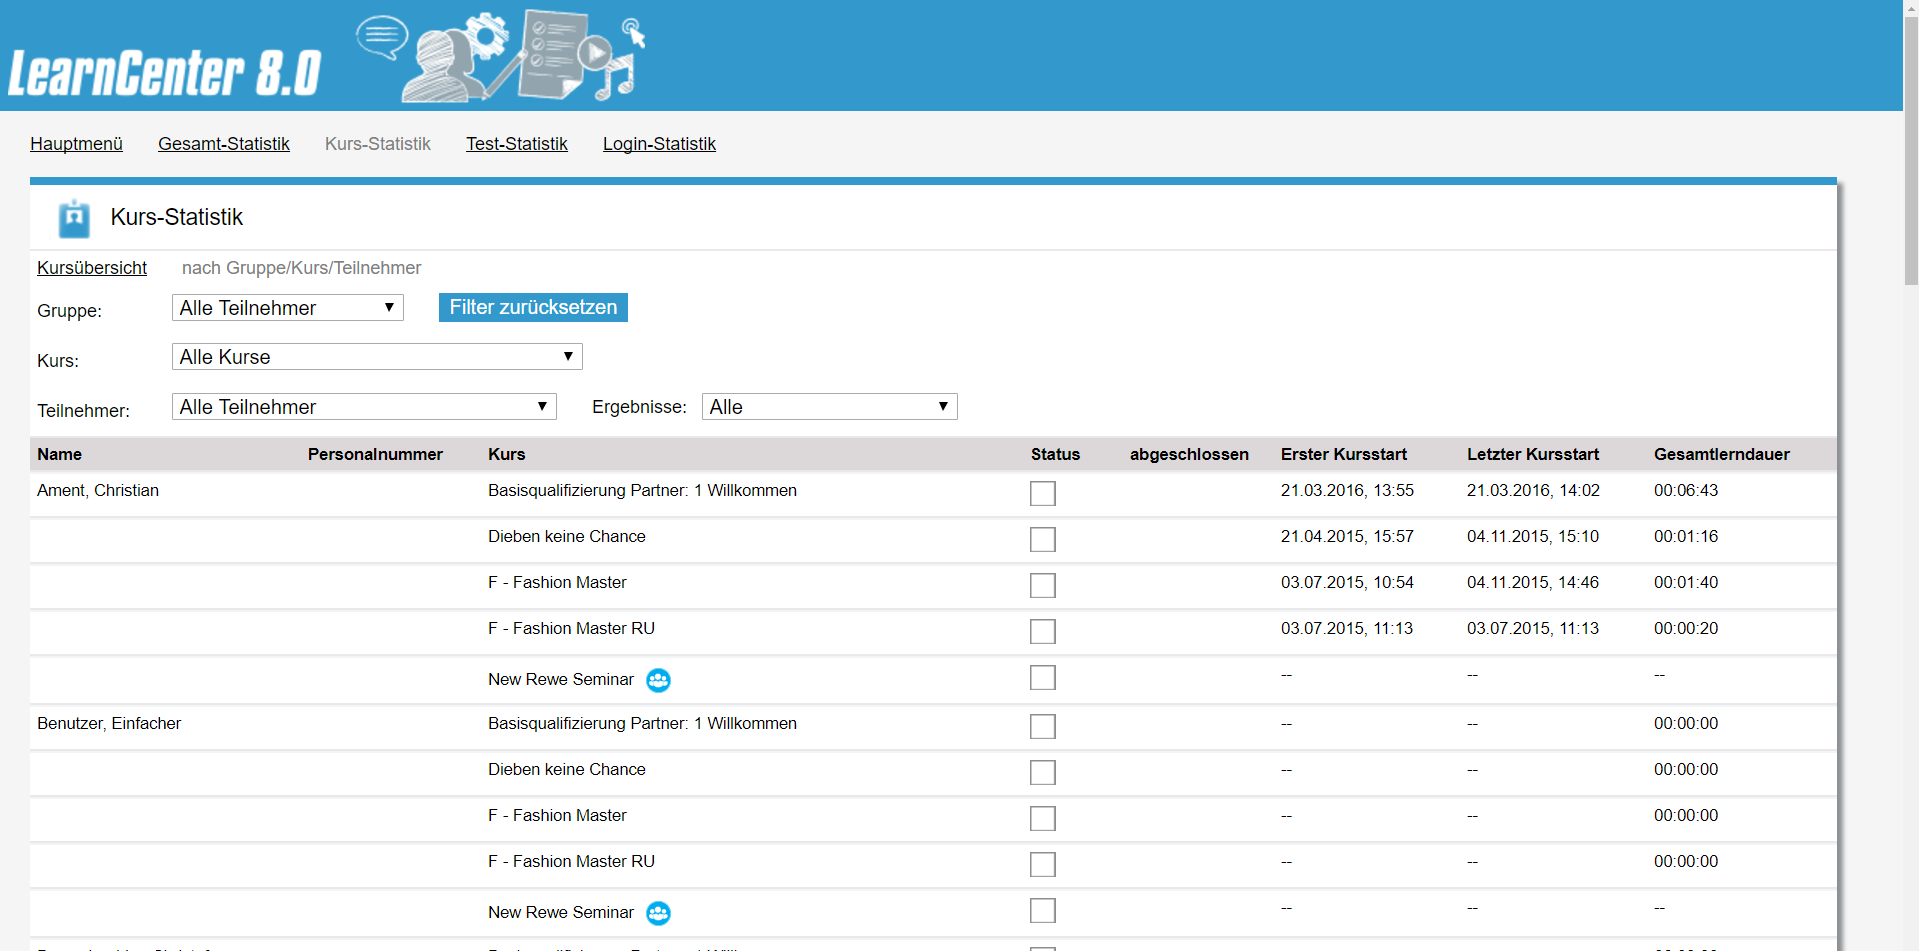
\includegraphics[width=\textwidth]{screenshots/estadisticas.png}
		\caption{Vista de las estadísticas mostradas al administrador.} \label{fig:estadisticasAdmin}
	\end{center}
\end{figure}

\begin{figure}[h]
	\begin{center}
		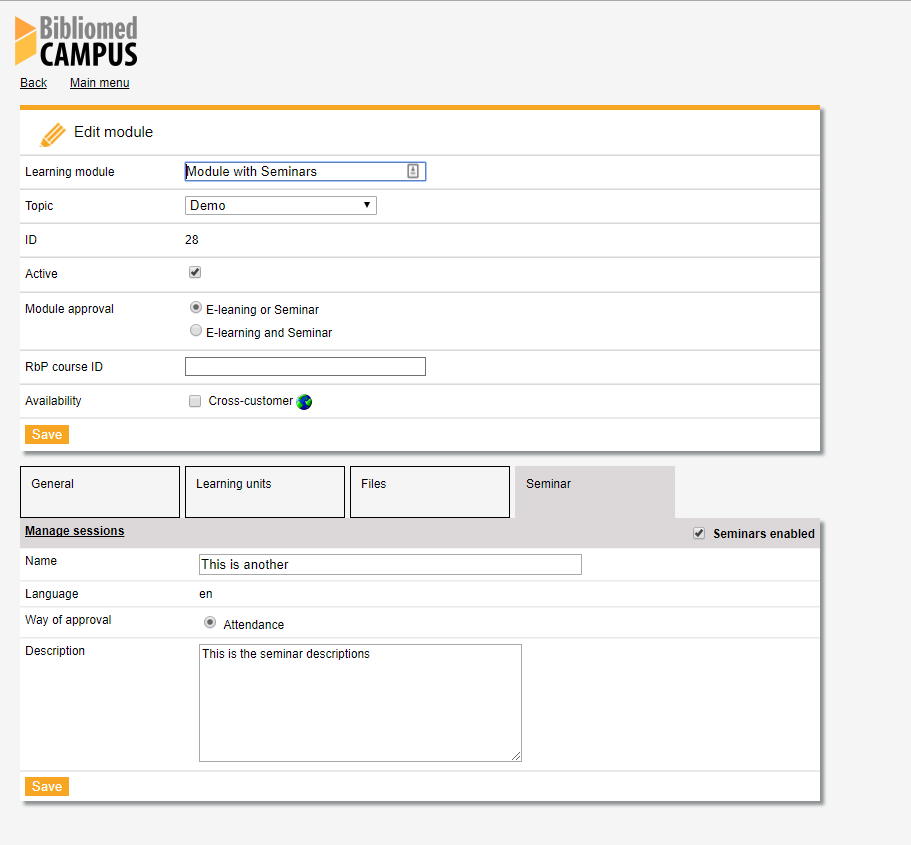
\includegraphics[width=\textwidth]{screenshots/bibliomed_adaptacion.png}
		\caption{Vista de la adaptación hecha para la creación de seminarios en el SGA de Bibliomed.} \label{fig:creacionSeminarioBibliomed}
	\end{center}
\end{figure}

\begin{figure}[h]
	\begin{center}
		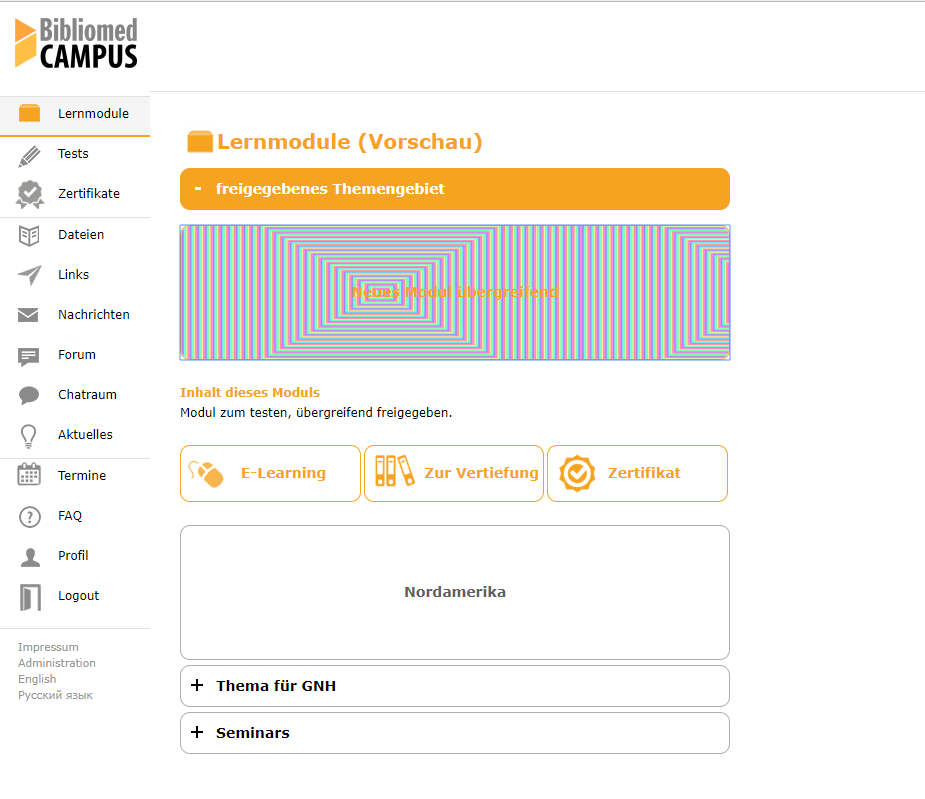
\includegraphics[width=\textwidth]{screenshots/bibliomed_viejo.png}
		\caption{Vista de cursos disponibles para el aprendiz antes de la integración de el módulo de seminarios en el SGA de Bibliomed.} \label{fig:bibliomedViejo}
	\end{center}
\end{figure}

\begin{figure}[h]
	\begin{center}
		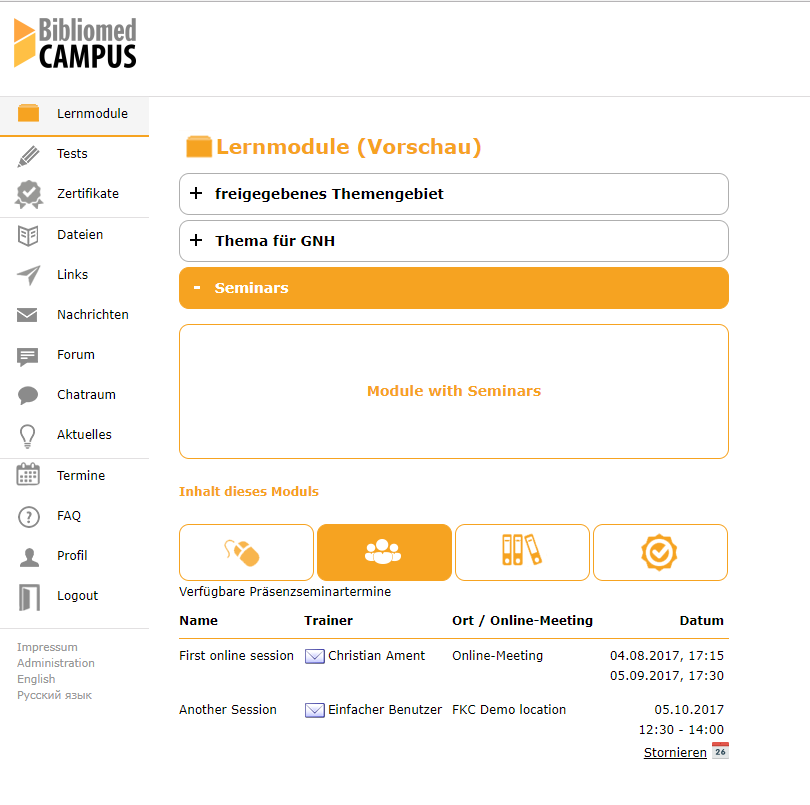
\includegraphics[width=\textwidth]{screenshots/bibliomed_reservar_sesion.png}
		\caption{Vista de una sesión reservada en el SGA de Bibliomed.} \label{fig:reservarSesionBiliomed}
	\end{center}
\end{figure}













